\chapter{FRAMEWORK AND SYSTEM DESIGN}

%------------------------------------------------------------------
% 3.1  Design Overview
%------------------------------------------------------------------
\section{Design Overview}

\begin{spacing}{1.5}
The deepfake detection system is built around a three-model ensemble that analyses every uploaded image through three independent detectors simultaneously --- a Vision Transformer for global pattern recognition, F3Net for frequency-domain artefact analysis, and EfficientNet-B4 for facial texture forensics. Each detector is specialised for a different class of manipulation signal, and their outputs are merged through a confidence-weighted fusion layer to produce a single, calibrated verdict.

The rationale for this ensemble design is straightforward: different synthesis methods leave different types of traces. A GAN-generated face tends to produce distinctive high-frequency artefacts in DCT space that are largely invisible spatially, while a face-swap video will show subtle texture discontinuities at the blend boundary that a frequency-domain model would miss. By running all three detectors in parallel and weighting them by their individual AUC-based reliability, the system is more robust than any single model and catches a wider range of manipulation types.

The system is split into two tiers: a FastAPI backend that handles model loading, inference, heatmap generation, and result serialisation; and a React/Vite frontend that provides the user interface, progress feedback, and interactive result visualisation.
\end{spacing}

%------------------------------------------------------------------
% 3.2  System Architecture
%------------------------------------------------------------------
\section{System Architecture}

%------------------------------------------------------------------
\subsection{High-Level Design}
%------------------------------------------------------------------

\begin{spacing}{1.5}
The system is organised into four layers that together cover the full request lifecycle from user interaction down to model inference and response delivery (Fig.\,\ref{c3:fig1}).

\begin{enumerate}
  \item \textbf{Presentation Layer:} A React web application (port 3000) built with Vite and TypeScript. Provides drag-and-drop image upload, live progress feedback, and an interactive results view with heatmap overlays, per-model vote table, and plain-language explanations.

  \item \textbf{API Layer:} A FastAPI server (port 8000) that exposes REST endpoints for health checking, image detection, and heatmap retrieval. Handles file validation, temporary storage, and pipeline orchestration.

  \item \textbf{Detection Pipeline:} The core inference logic. Pre-processes the uploaded image and dispatches it to all three models in parallel. Collects their probability outputs, applies per-model Platt-scaling calibration, fuses the results, and generates an ensemble heatmap.

  \item \textbf{Model Layer:} Three independent neural networks, each with its own preprocessing, forward pass, and saliency map extraction. All models are loaded eagerly at startup and held in memory to avoid per-request initialisation latency.
\end{enumerate}
\end{spacing}

\begin{figure}[htbp]
  \centering
  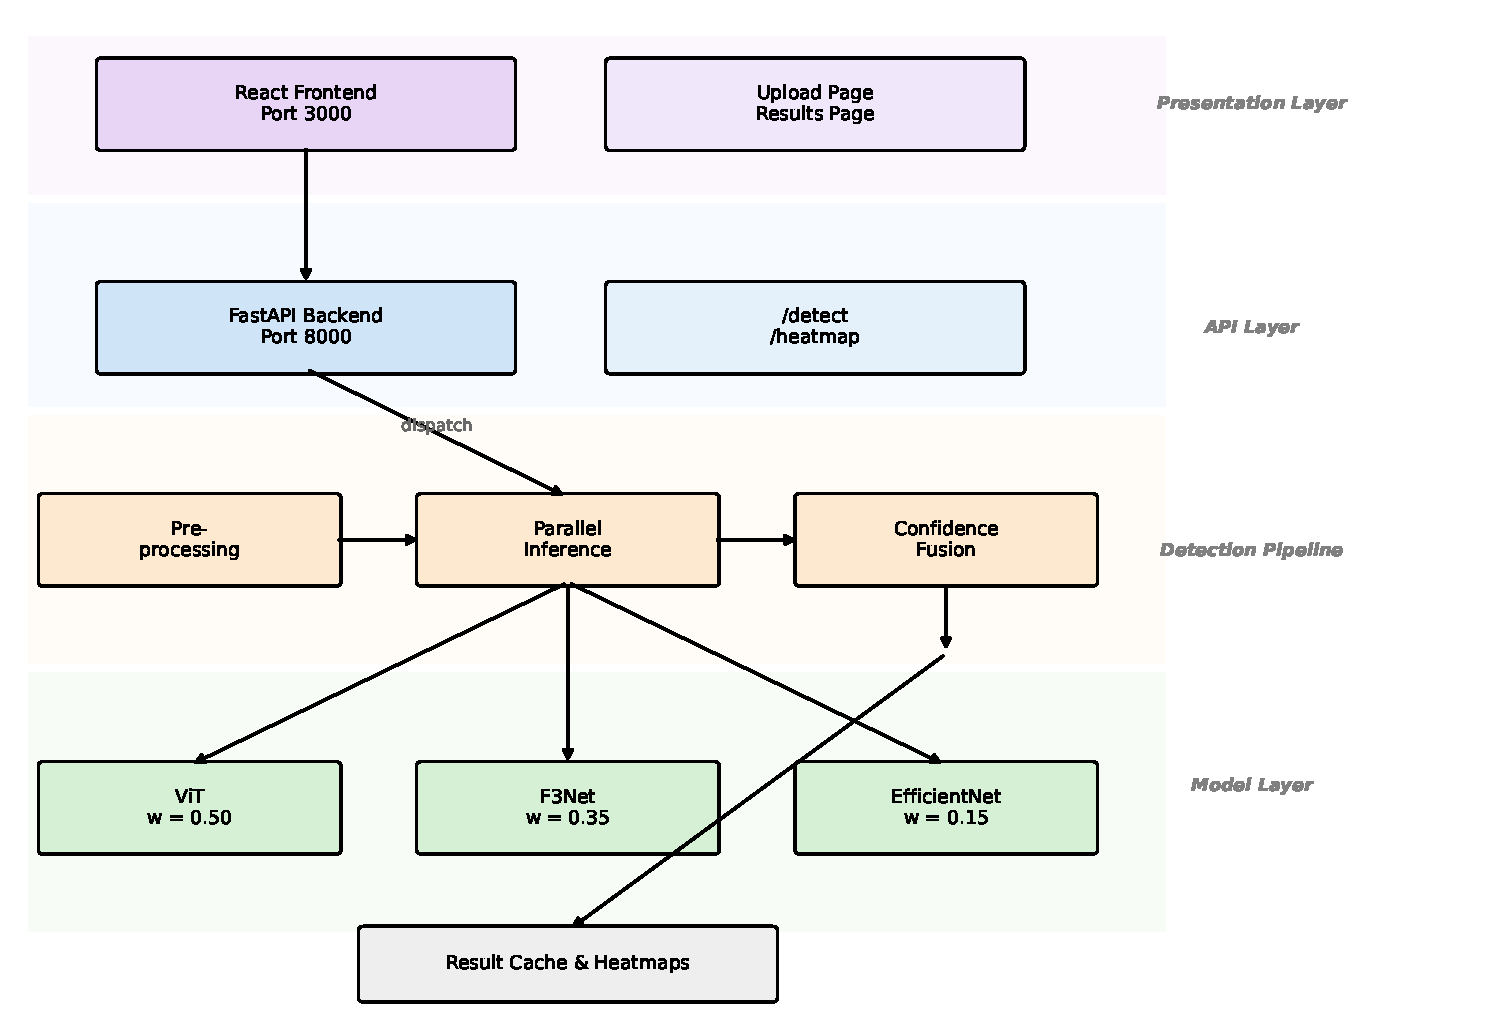
\includegraphics[width=0.88\textwidth]{figures/arch.pdf}
  \caption{Deepfake Detection System Architecture Diagram}
  \label{c3:fig1}
\end{figure}

%------------------------------------------------------------------
\subsection{Model Ensemble and Fusion Strategy}
%------------------------------------------------------------------

\begin{spacing}{1.5}
The detection pipeline runs three specialist models in parallel. Each model is pre-trained and fine-tuned on deepfake datasets, then calibrated with Platt scaling before its probability is used in fusion.

\noindent\textbf{Vision Transformer (ViT).}\quad
The primary model (fusion weight 0.50), based on \texttt{vit-base-patch16-224} fine-tuned on approximately 200,000 real and AI-generated samples. The model splits the input into 16$\times$16 pixel patches and processes them through multi-head self-attention, capturing long-range manipulation signatures across the full image. Saliency maps are derived from CLS-to-patch attention weights in the final transformer layer.
\begin{itemize}
  \item Input: 224$\times$224 RGB \quad|\quad Parameters: 86M \quad|\quad AUC: 0.999
  \item Fusion weight: 0.50 (face detected), 0.55 (no face)
\end{itemize}

\noindent\textbf{F3Net --- Frequency-Domain Analysis.}\quad
Combines a ResNet-50 spatial backbone with a frequency-feature fusion branch (FAD\,+\,LFS) to detect DCT-domain artefacts left by neural image generators. Both branches process the image in parallel; their feature maps are fused before the binary classification head. GradCAM is applied at the fusion point for heatmap generation.
\begin{itemize}
  \item Input: 380$\times$380 RGB \quad|\quad Preprocessing: DCT decomposition \quad|\quad AUC: 0.958
  \item Fusion weight: 0.35 (face detected), 0.40 (no face) \quad|\quad Weights: \texttt{f3net\_binary\_best.pth}
\end{itemize}

\noindent\textbf{EfficientNet-B4 --- Facial Texture Forensics.}\quad
Targets facial texture irregularities typical of face-swap deepfakes. MediaPipe first locates and crops the largest face; the crop is then classified by EfficientNet-B4. If no face is detected, the full image is used with a significantly reduced fusion weight. GradCAM++ is applied to the final convolutional block.
\begin{itemize}
  \item Input: 380$\times$380 RGB face crop \quad|\quad Parameters: 19M \quad|\quad AUC: 0.91
  \item Fusion weight: 0.15 (face detected), 0.05 (no face) \quad|\quad Weights: \texttt{efficientnet\_binary.pth}
\end{itemize}

\noindent\textbf{Confidence Fusion and Verdict Thresholds.}\quad
After each model produces a calibrated fake probability, the three scores are merged using confidence-weighted averaging:

\begin{equation}
  \text{final\_score} = \sum_{i} w_i \times \text{fake\_prob}_i
  \label{eq:fusion}
\end{equation}

where $w_i$ is the normalised AUC-based weight for model $i$ and $\text{fake\_prob}_i$ is its Platt-scaled softmax output. The final verdict is determined by thresholding the fused score:
\begin{itemize}
  \item \textbf{Fake:}\quad final\_score $\geq 0.62$
  \item \textbf{Uncertain:}\quad $0.38 <$ final\_score $< 0.62$
  \item \textbf{Real:}\quad final\_score $\leq 0.38$
\end{itemize}

The uncertain band (0.38--0.62) covers cases where the models disagree or confidence is low; these are surfaced to the user rather than assigned a definitive verdict. Fig.\,\ref{c3:fig3} illustrates the fusion with a concrete numerical example.
\end{spacing}

\begin{figure}[htbp]
  \centering
  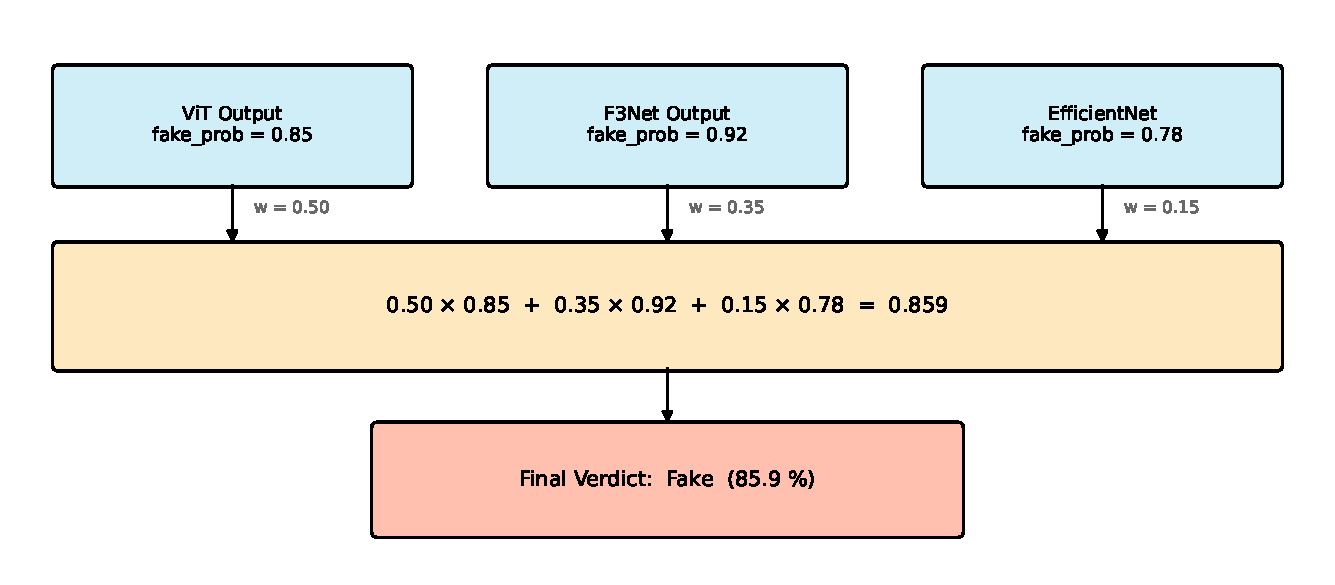
\includegraphics[width=0.90\textwidth]{figures/fusion.pdf}
  \caption{Confidence Fusion Process With Example}
  \label{c3:fig3}
\end{figure}

%------------------------------------------------------------------
\subsection{Frontend and Backend Components}
%------------------------------------------------------------------

\begin{spacing}{1.5}
The backend exposes three REST endpoints (Table\,\ref{c3:tab1}). All requests and responses use JSON; images are submitted as multipart form data on the \texttt{/detect} endpoint. All three models are loaded eagerly at application startup --- EfficientNet ($\approx$90\,MB), F3Net ($\approx$110\,MB), and ViT ($\approx$350\,MB from HuggingFace Hub) --- giving a cold-start time of 15--30 seconds and zero per-request initialisation latency.
\end{spacing}

\renewcommand{\arraystretch}{1.3}
\begin{table}[htbp]
  \centering
  \begin{tabular}{|l|l|p{5.5cm}|}
  \hline
  \textbf{Method} & \textbf{Endpoint} & \textbf{Description} \\
  \hline
  GET  & \texttt{/api/v1/health}  & Health check --- returns \texttt{\{"status":"ok"\}} \\
  \hline
  POST & \texttt{/api/v1/detect}  & Accept image upload; returns full detection JSON \\
  \hline
  GET  & \texttt{/api/v1/results/\{id\}/heatmap/\{model\}} & Stream PNG heatmap overlay for a model \\
  \hline
  \end{tabular}
  \caption{Backend API Endpoints}
  \label{c3:tab1}
\end{table}

\begin{spacing}{1.5}
The React frontend is structured around two page-level components --- \textit{UploadPage} (file selection, preview, submit) and \textit{ResultsPage} (verdict, votes, heatmaps, explanations) --- backed by the supporting components listed in Table\,\ref{c3:tab2}. Table\,\ref{c3:tab3} summarises the full technology stack used across both tiers.
\end{spacing}

\renewcommand{\arraystretch}{1.3}
\begin{table}[htbp]
  \centering
  \begin{tabular}{|l|p{7.5cm}|}
  \hline
  \textbf{Component} & \textbf{Purpose} \\
  \hline
  VerdictBanner    & Displays final verdict with colour-coded confidence percentage ring \\
  \hline
  ModelVoteTable   & Per-model fake probability, inference time, and fusion weight \\
  \hline
  HeatmapViewer    & Switchable heatmap overlays (Ensemble / ViT / F3Net / EfficientNet) with opacity slider \\
  \hline
  ExplanationsCard & Ordered plain-language findings from each detector \\
  \hline
  \end{tabular}
  \caption{Frontend UI Components}
  \label{c3:tab2}
\end{table}

\renewcommand{\arraystretch}{1.3}
\begin{table}[htbp]
  \centering
  \begin{tabular}{|l|l|l|}
  \hline
  \textbf{Component}        & \textbf{Technology}            & \textbf{Version} \\
  \hline
  Backend Framework         & FastAPI                        & 0.111.0 \\
  Backend Server            & Uvicorn                        & 0.30.0  \\
  ML Framework              & PyTorch                        & $\geq$2.0.0 \\
  Image Processing          & OpenCV                         & 4.9.0   \\
  Face Detection            & MediaPipe                      & 0.10.14 \\
  Transformer Models        & HuggingFace Transformers       & Latest  \\
  \hline
  Frontend Framework        & React                          & 18.3.1  \\
  Build Tool                & Vite                           & 5.4.21  \\
  State Management          & Zustand                        & 4.5.2   \\
  HTTP Client               & Axios                          & 1.7.2   \\
  CSS Framework             & Tailwind CSS                   & 3.x     \\
  \hline
  \end{tabular}
  \caption{Technology Stack}
  \label{c3:tab3}
\end{table}

%------------------------------------------------------------------
% 3.3  Workflow and Processing Pipeline
%------------------------------------------------------------------
\section{Workflow and Processing Pipeline}

%------------------------------------------------------------------
\subsection{Image Processing}
%------------------------------------------------------------------

\begin{spacing}{1.5}
When an image is uploaded, the backend loads it with OpenCV and normalises it to RGB. It is then dispatched simultaneously to all three models --- each resizes and preprocesses the input to its required resolution independently (224$\times$224 for ViT; 380$\times$380 for F3Net and EfficientNet). Each model runs a forward pass, extracts its saliency map, and returns a calibrated fake probability. The three probabilities are fused using the weighted average in Eq.\,\eqref{eq:fusion}. An ensemble heatmap is generated by averaging the three individual saliency maps, and a plain-language explanation is assembled from per-model findings. The backend then serialises and returns the full result JSON. On CPU hardware, the complete image pipeline completes in 1200--2000\,ms; GPU acceleration reduces this to 400--800\,ms.
\end{spacing}

%------------------------------------------------------------------
\subsection{Video Processing}
%------------------------------------------------------------------

\begin{spacing}{1.5}
For video inputs, keyframes are extracted at one-second intervals using scene-change detection, reducing the number of frames to analyse by approximately 90\,\% compared to processing every frame. Each keyframe is processed independently through the same image detection pipeline described above. The per-frame fake probabilities are then analysed for temporal consistency --- abrupt transitions between high and low fake-probability frames are flagged as potential splice or face-swap artefacts. A final video-level verdict is derived by majority voting across keyframe verdicts, weighted by confidence. Fig.\,\ref{c3:fig2} shows the complete branching workflow covering both media types.
\end{spacing}

\begin{figure}[htbp]
  \centering
  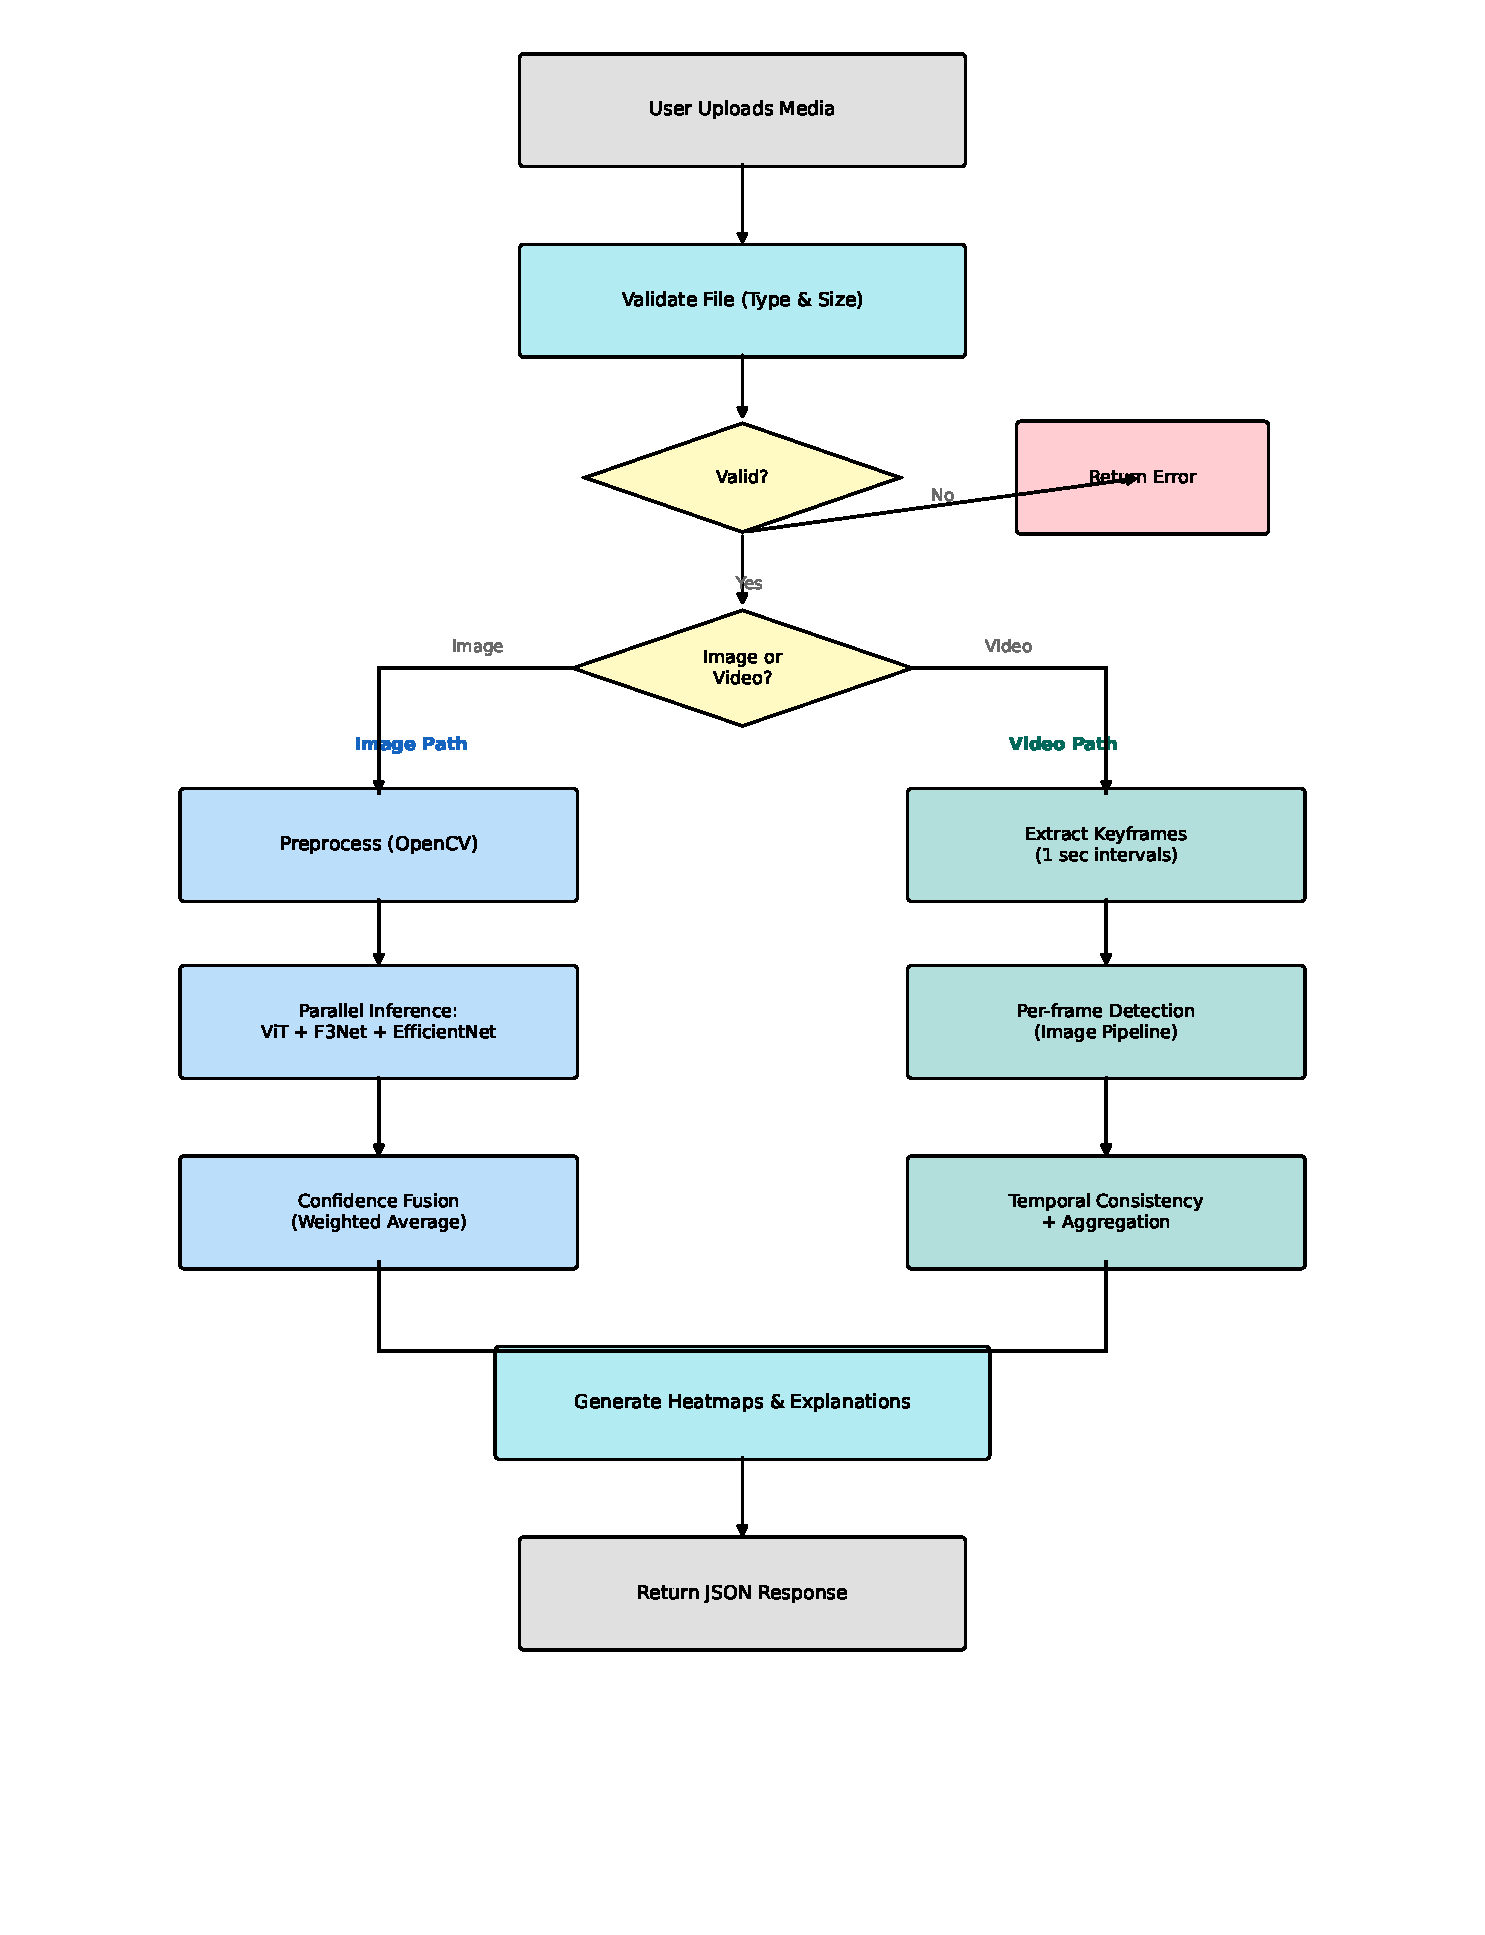
\includegraphics[width=0.82\textwidth]{figures/workflow.pdf}
  \caption{Unified Detection Workflow --- Image and Video Paths}
  \label{c3:fig2}
\end{figure}

%------------------------------------------------------------------
\subsection{User Interaction Flow}
%------------------------------------------------------------------

\begin{spacing}{1.5}
The frontend guides the user through a seven-step journey from upload to results. The UploadPage accepts a drag-and-dropped or browsed file and shows a preview before submission. Clicking \textit{Analyse Image} triggers a POST to \texttt{/api/v1/detect} and displays a progress indicator while the backend runs inference. On completion, the frontend automatically navigates to the ResultsPage, which renders the verdict banner, the per-model vote table, the interactive heatmap viewer, and the explanation card. The user can switch between model heatmaps (Ensemble, ViT, F3Net, EfficientNet), adjust overlay opacity with a slider, and click \textit{New Image} to restart the flow. Fig.\,\ref{c3:fig4} shows the end-to-end user journey.
\end{spacing}

\begin{figure}[htbp]
  \centering
  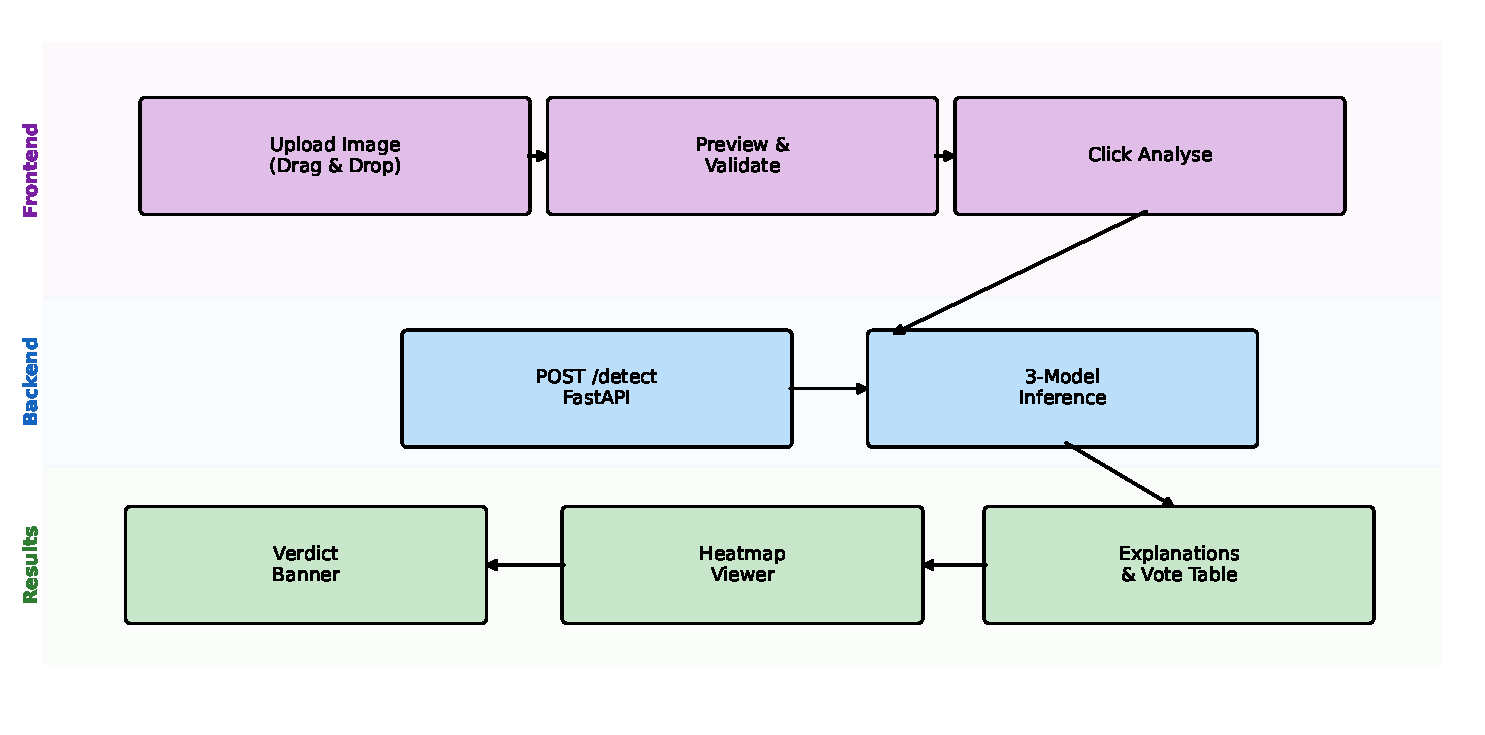
\includegraphics[width=0.90\textwidth]{figures/userflow.pdf}
  \caption{User Interaction Flow --- Frontend, Backend, and Results}
  \label{c3:fig4}
\end{figure}

%------------------------------------------------------------------
% 3.4  Summary
%------------------------------------------------------------------
\section{Summary}

\begin{spacing}{1.5}
This chapter described the framework and architecture of the deepfake detection system. The design centres on a three-model ensemble --- ViT for global spatial patterns, F3Net for frequency-domain artefacts, and EfficientNet-B4 for facial texture forensics --- whose outputs are merged through a calibrated, AUC-weighted confidence fusion to produce a single verdict. The system is split into a FastAPI backend that handles inference and heatmap generation, and a React frontend that provides interactive visualisation of results. The unified processing pipeline supports both image and video inputs, with video analysis using keyframe sampling and temporal consistency checking to keep computation tractable. Together, these components form a robust, interpretable deepfake detection tool capable of flagging manipulated media across a range of synthesis methods.
\end{spacing}
